\chapter{Neural Net Based Electronics Response Modeling}
\label{chap:elect_resp}

\section{Introduction}
As discussed in chapter \ref{chap:detectors}, HPGe detectors provide excellent energy resolution and good waveform-shape–based event identification, making them critical for low-background physics searches such as $0\nu\beta\beta$ searches. However, the signal from the HPGe detector must pass through an electronic readout chain consisting of components such as a pre-amplifier, filtering stages, and digitization. These electronics transform the signal in ways that can distort waveform shapes, alter the rise time, and add overshoots/undershoots or baseline shifts. Accurate modeling of this transformation is crucial for producing realistic pulse shape simulations.

This chapter begins with an overview of typical HPGe detector readout electronics. It is followed by an overview of {\Ltwo}  electronics and how electronics introduce distortions in waveforms, called the electronics response. This is followed by challenges in modeling the electronics response and a neural network approach to it.

\section{{\Ltwo} Readout Electronics}

{\Ltwo} uses a resistive feedback charge sensitive amplifier (CSA) to minimize noise and achieve a low radioactive background, as shown in Figure \ref{ch6_fig_l200_elec_model}. The first stage is termed the Low Mass Front End (LMFE). LMFE is placed inside the liquid argon cryostat of the experiment, only a few millimeters from the point of contact of each HPGe detector \cite{Willers_2020}. LMFE is therefore constructed with high radiopure materials with tolerance typically on the order of $1\mu$ Bq per channel. LMFE builds upon one developed by {\MJD} and is produced using Suprasil substrates, titanium-gold (TiAu) traces, an in-die junction field effect transistor (JFET, Moxtek MX11), and thin-film amorphous germanium feedback resistors that can operate at cryogenic temperatures. The first stage is connected to the second stage using four ultra-pure Axon pico-coaxial cables.

\begin{figure}[!htb]%[htb!]
  %[trim={left bottom right top},clip]
    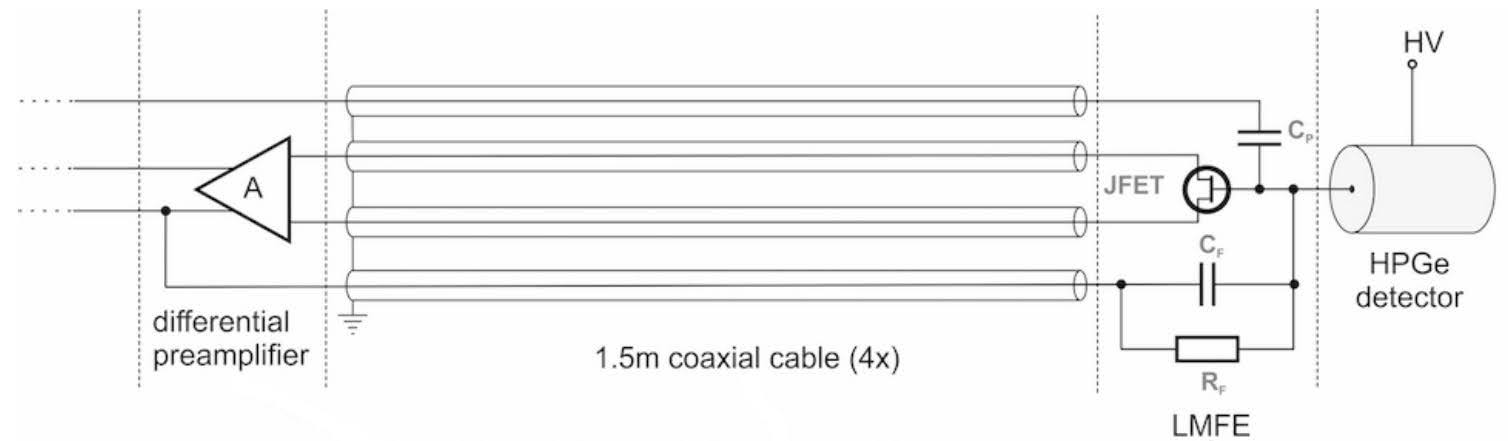
\includegraphics[width=0.99\linewidth,trim={1pc 0pc 1pc 0pc},clip]{ch6/figs/l200_elec_diagram.jpg}
    \caption{A Schematic of the {\Ltwo} signal readout chain.\cite{Willers_2020}}
   \label{ch6_fig_l200_elec_model}
\end{figure}

\begin{figure}[!htb]%[htb!]
  %[trim={left bottom right top},clip]
  \centering
    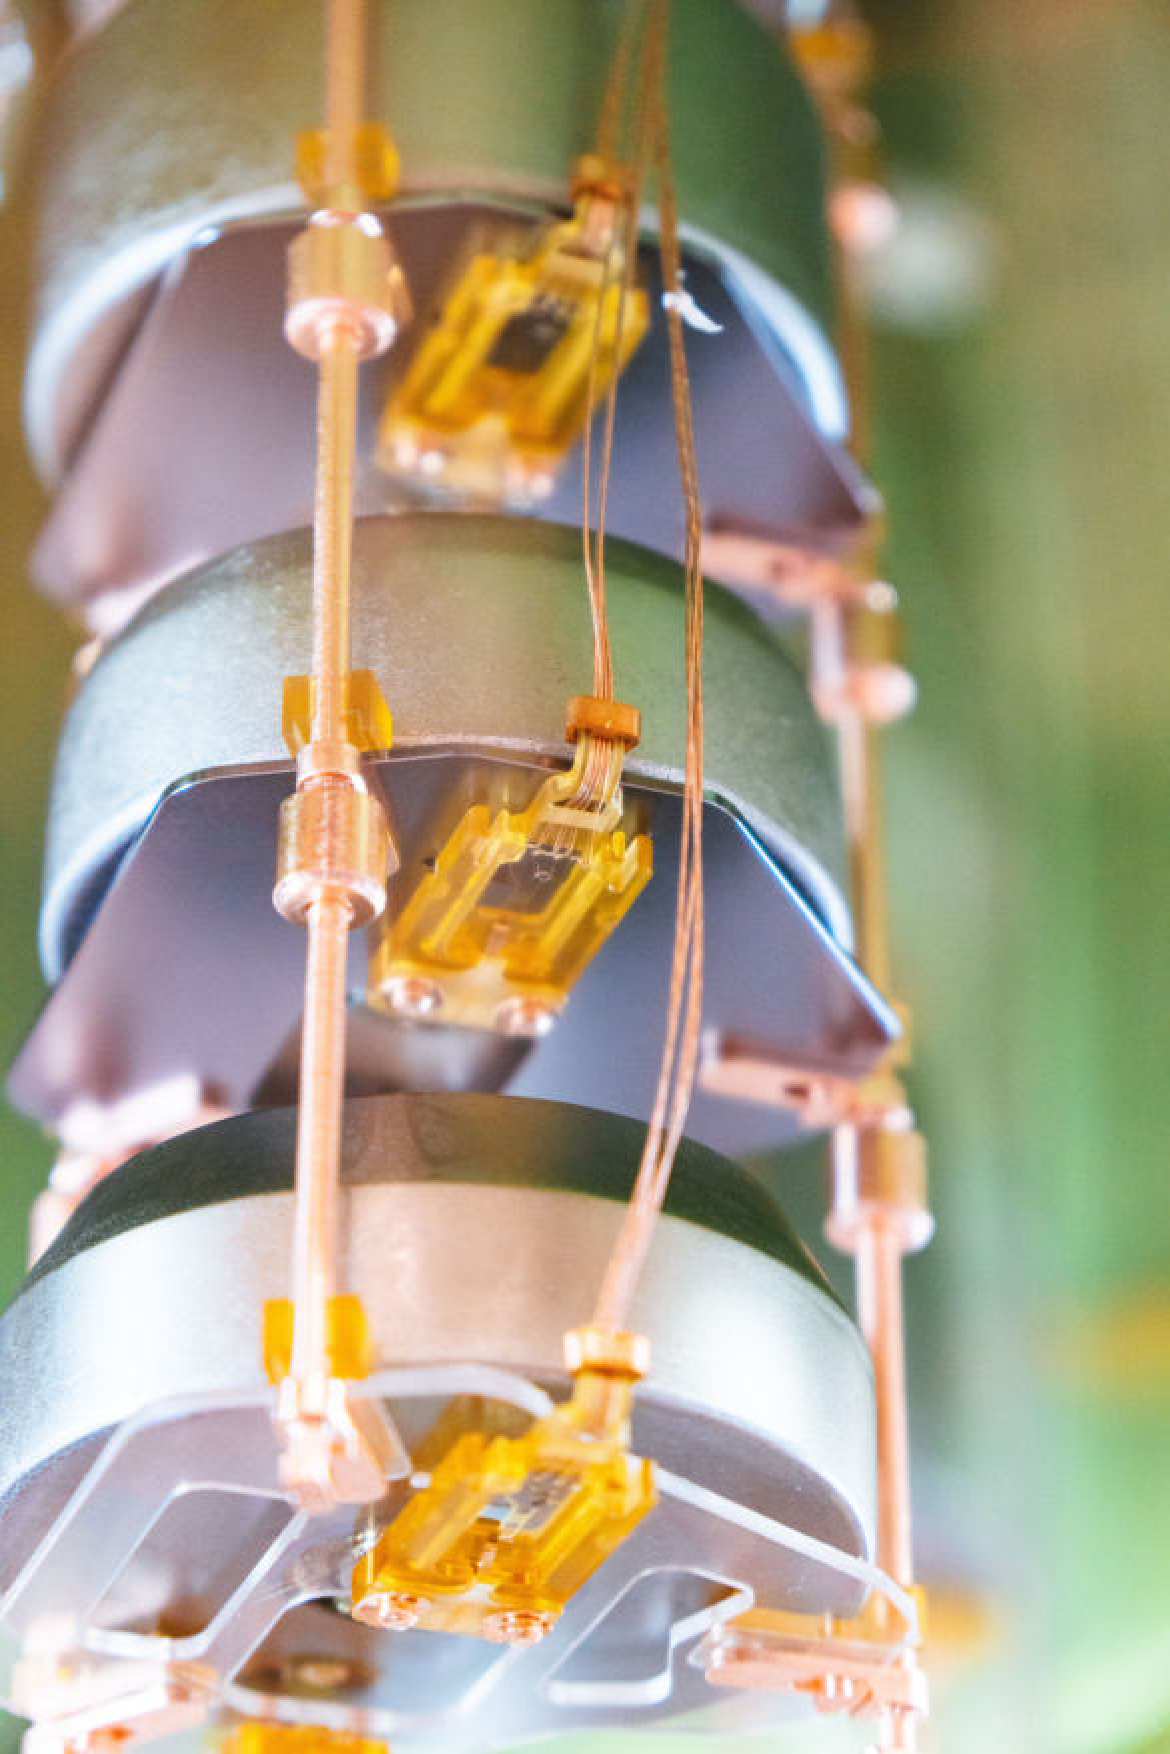
\includegraphics[width=0.32\linewidth,trim={1pc 0pc 1pc 0pc},clip]{ch6/figs/lmfe_det.pdf}
    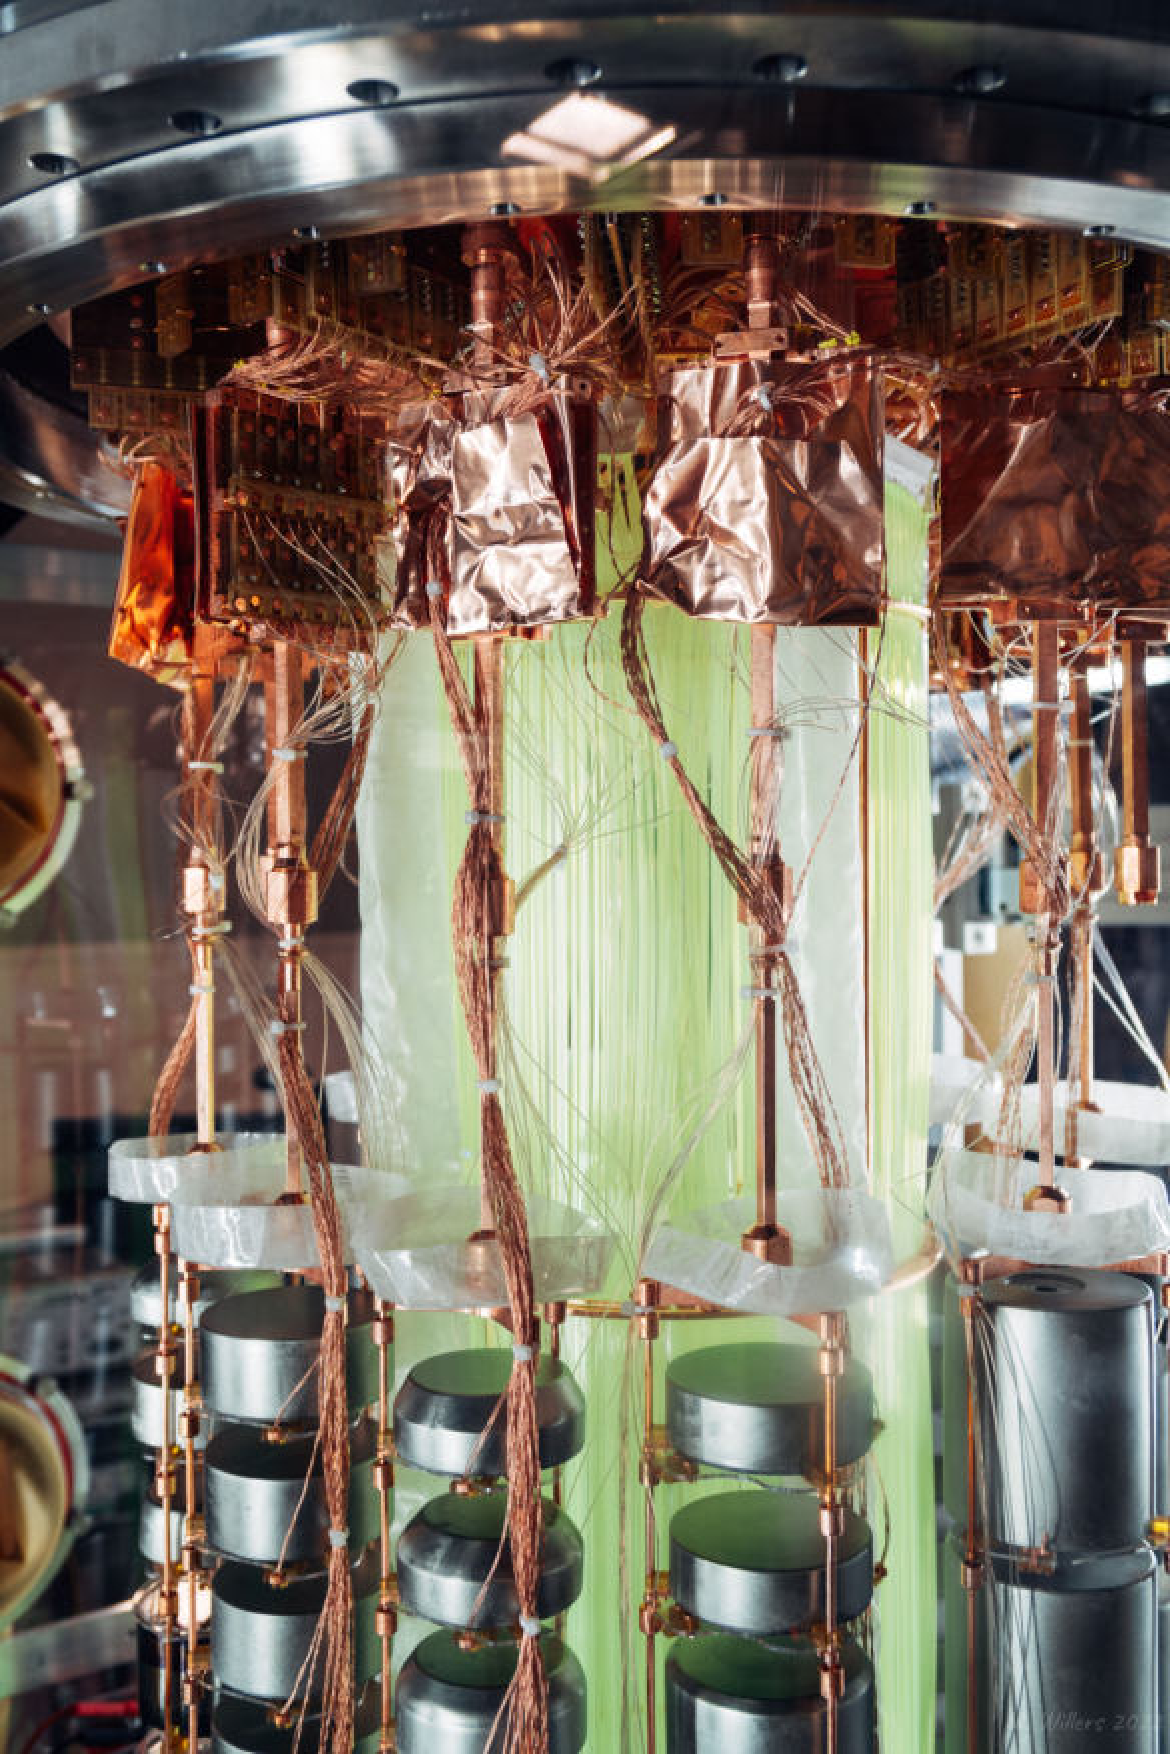
\includegraphics[width=0.32\linewidth,trim={1pc 0pc 1pc 0pc},clip]{ch6/figs/front_elect.pdf}
    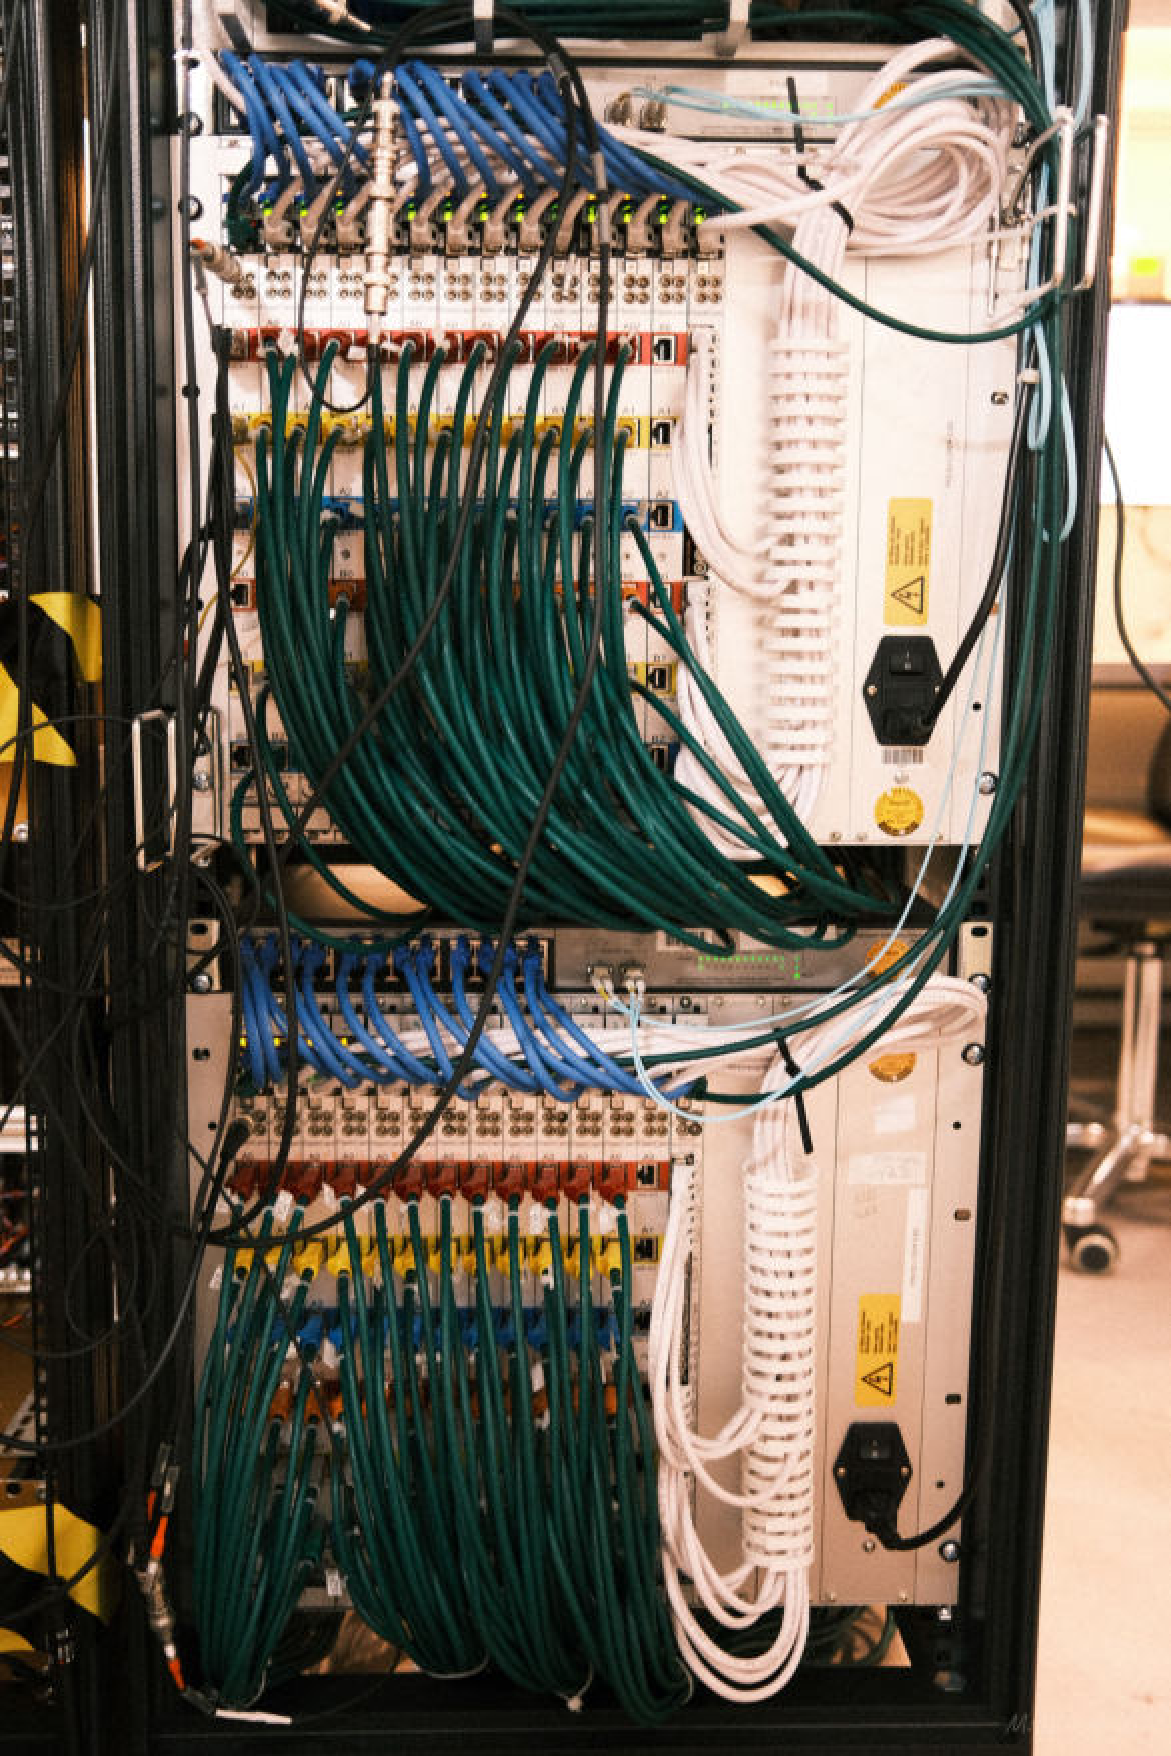
\includegraphics[width=0.32\linewidth,trim={1pc 0pc 1pc 0pc},clip]{ch6/figs/daq_crate.pdf}
    \caption{Picture of the front end electronics of {\Ltwo}. Left show close up of the detector with the LMFE, middle shows the detector strings front end electronics, the CC4s are located directly at the top. Below them are the connectors for the high voltage cable. Right shoes the Flashcam crates in the DAQ rack. Photo: Michael Willers}
   \label{ch6_fig_l200_elec_model_real}
\end{figure}


The second amplifier is based on a folded cascode arrangement and is located $30$ -$150$ cm from the detector to provide additional gain and convert the signal to a differential output. This stage can tolerate slightly higher radioactivity levels of $50\mu$ Bq per channel and is built using commercial screened surface mount components on Kapton circuit boards called the CC4. The second stage is connected to the data acquisition system using a $\thicksim 10$ m long transmission line. An active buffer called Head Electronics receives the signals from the second stage. This adjusts offsets and gain while providing impedance matching. Finally, the signals are fed into a FlashCam where the signal is digitized and stored for analysis.

Together, these design choices enable sub-3 keV FWHM energy resolution in the ROI at $Q_{\beta\beta}$ 2039 keV while minimally contributing to the overall radioactive background. They also enable a fast rise time of $\thicksim 0.100$ ns which allows pulse shape discrimination of the signals. In addition, they have a high range of up to 10 MeV that enables measurement of high-energy alpha decays, which would provide additional information for background modeling.

\section{Electronics Influence on Waveforms}

Despite careful design and component selection, the LEGEND-200 electronics chain inevitably modifies the detector’s raw current signals. Figure~\ref{fig:sim_data_comp} shows some of these effects by comparing a simulated waveform (blue) with a corresponding real data waveform (red).

The baseline is the region before $t_0$, the start of the waveform. Ideally, this baseline should remain near a stable DC offset determined by the quiescent operating point of the preamplifier. Two factors can shift or tilt the baseline. First, a slow high-pass filter effect (on the order of milliseconds) arises from the capacitive coupling between the first and second preamplifier stages. Second, if events occur in rapid succession, the tail of one waveform may not fully decay before the next arrives, causing the baseline to drift or undershoot. These shifts become especially noticeable at higher rates, leading to soft pile-up where partial overlap deforms the apparent starting level of subsequent waveforms. 

The rising edge, shown in the orange region, is the most visible part of the waveform resulting from the movement of holes and electrons from the energy deposition. The long cable and folded-cascode amplifier stages introduce a finite bandwidth, effectively acting as a low-pass filter that damps the highest-frequency components. As a result, the observed rising edge in real data tends to be broader and smoother than in simulations. 

The RC decay tail (light blue region) develops from the CSA feedback network in the LMFE, where the detector current is integrated on a feedback capacitor and slowly discharged by the feedback resistor. The second stage of amplification has a shorter differentiator-like time constant, further modifying the decay shape seen in the data. Together, these processes create a waveform with multiexponential decay. 


In general, the three waveform regions, the baseline, the rising edge, and the tail, are each influenced by different parts of the LEGEND-200 electronic chain. Circuit simulations such as SPICE can reproduce some of the bulk features, but minute responses such as parasitic inductance, JFET nonlinearity, or thermal drifts are hard to model.

\begin{figure}[!htb]%[htb!]
  %[trim={left bottom right top},clip]
    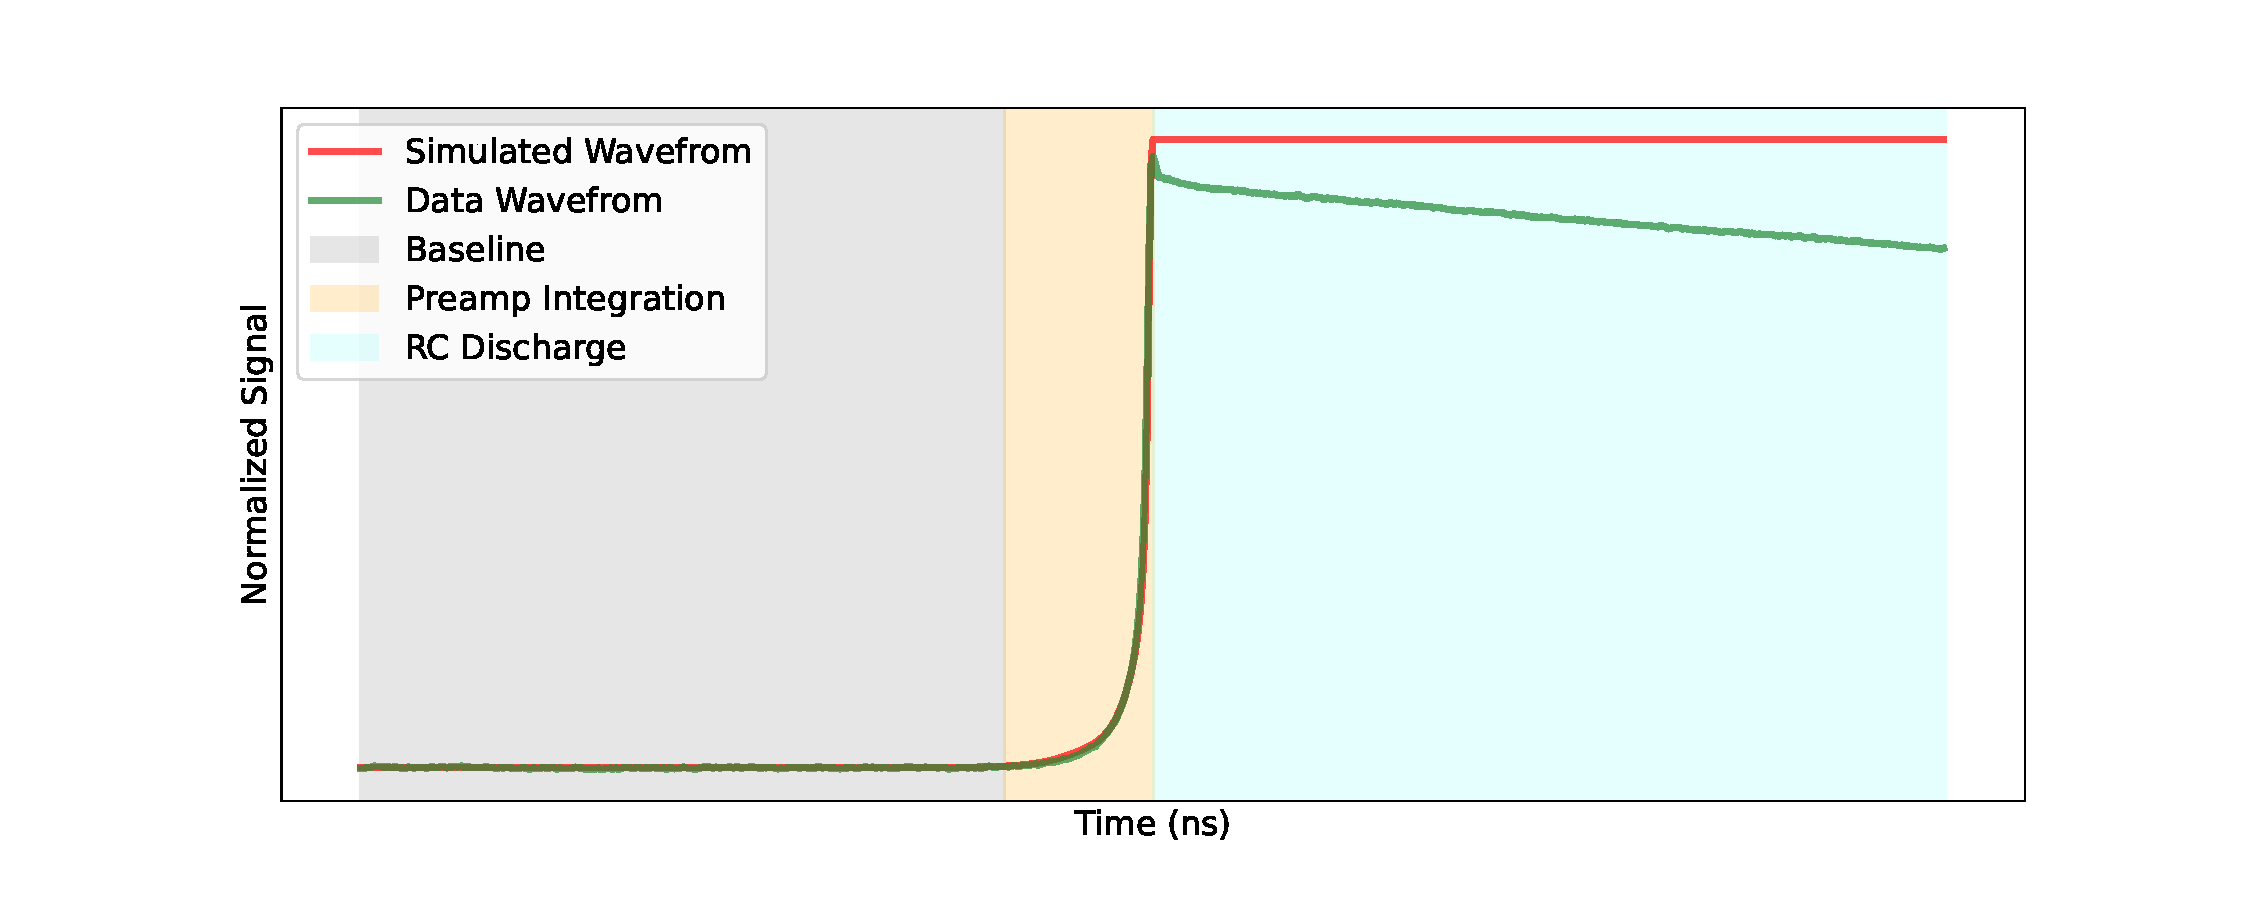
\includegraphics[width=\linewidth,trim={4cm 0pc 3.5cm 0pc},clip]{ch6/figs/wf_comp_sim_data.pdf}
    \caption{Comparison of a simulated waveform with a real data waveform. The two pulses were randomly sampled from datasets and are aligned for clarity. Three components of the waveforms are labeled The data pulses contains electronics effects such as RC decay tail, electronics noise and preamp integration.}
    \label{fig:sim_data_comp}
\end{figure}

\section{Challenges in Modeling Electronics Response}

Pulse shape simulation aims at generating waveforms that are similar to the actual detector waveforms. Having a direct mapping between a simulated waveform and its corresponding incident particle would enable applying the same cuts to the simulations as data. This would help us understand the efficiency of cuts such as multi-site cuts ~\cite{AvsE}.  

A frequency-dependent response function must be added to the simulations to reproduce the detector response. The electronic transfer function describes the series of linear transformations on the detector output signal by the readout electronic components. The electron response is typically derived from the circuit response to a step function input. However, the experimental conditions commonly used in low-background and cryogenic experiments, such as long cable runs and extended amplification chains, make it difficult to generate waveforms close to the detector. This poses significant challenges in measuring the electronics response directly. Figure \ref{ch6_fig_l200_elec_model_real} shows the front-end electronics of {\Ltwo}, a contrast to Fig. \ref{ch6_fig_l200_elec_model} showing how in practice the electronics setup can be quite complicated.

Although simulations can account for some of these effects, they are inherently limited by assumptions. These assumptions often fail to capture the complexities of real-world behavior, such as detector-specific anomalies, nonlinearity in the amplification chain, or subtle effects from experimental conditions. Furthermore, inaccuracies in simulation assumptions, such as incorrect drift velocity calculations in the electric field or oversimplified charge cloud dynamics, can exacerbate discrepancies between simulated and real detector waveforms. The result is a persistent mismatch between the simulated and measured waveforms, necessitating ad hoc corrections. 

Heuristic methods are often used to approximate the electronic response. Current experiments avoid detailed electronics modeling by calculating reconstruction features directly from Monte Carlo particle-interaction simulations, relying on heuristic methods to meet most of their simulation needs ~\cite{Ben_Thesis,Sam_Thesis}. These methods fall short in their ability to account for detector-by-detector variations and operational changes in experimental conditions, which can evolve over time. This lack of adaptability introduces systematic errors and limits the fidelity of pulse shape simulations.

Transfer Learning is an unsupervised learning approach to learn the translations between the simulated waveform and the corresponding detector waveform. In the next section, we present a new neural network model called Cyclic Positional U-Net~(CPU-Net) that allows learning the translations from the data and applying them to simulations without explicit programming.

\section{Machine Learning Based Electronics Modeling}
\subsection{Mathematical Formulism}
The task of learning the transfer function of electronics from data and adding them to the simulation can be reformulated under the transfer learning framework. The goal is to translate simulated waveforms into real waveforms by learning the differences between them.

In this approach, the source domain $\mathcal{D}_{Source}$ represents the simulated waveforms. It includes features of the simulated waveforms, such as energy, maximal current amplitude, tail slope, etc. These features form a feature space ($\mathcal{Y}$) and follow a probability distribution $(P(Y))$. The source task refers to the relationship between the reconstruction features $(Y)$ in the source domain and the simulated waveforms ($\mathcal{X}$). This is captured by the conditional distribution $P(X|Y)$, which describes how each parameter set $(Y)$ is assigned to a specific simulated waveform $(X)$. For instance, if we know the energy and rise time of a waveform, the source task models how these features produce a simulated waveform. Mathematically, we write the source domain as follows:

\begin{equation}
    \mathcal{D}_{Source}=\{\mathcal{Y},P(Y)\}\qquad 
    \label{eqn:source_domain}
\end{equation}
Then the reconstruction features are written as:
 \begin{equation}
     Y=\{\mathrm{E},I_{\mathrm{max}},c_{\mathrm{tail}}...\}\in \mathcal{Y}
 \end{equation}

The source task is written as:
\begin{equation}
    \mathcal{T}_{Source}=\{\mathcal{X},P(X|\mathcal{Y})\} \qquad X\in \mathcal{X}
    \label{eqn:source_task}
\end{equation}

Similarly, target domain $\mathcal{D}_{Target}$ represents the detector data waveform. It contains the feature space $\mathcal{Y'}$ whose elements follow the probability distribution $P(Y')$, $Y'$ are the reconstruction features of the detector waveforms $(X')$.

\begin{equation}
\mathcal{D}_{Target}=\{\mathcal{Y}',P(Y')\}
\end{equation}
\begin{equation}
\mathcal{T}_{Target}=\{\mathcal{X}',P(X'|\mathcal{Y}')\}
\end{equation}

Pulse shape simulation typically learns $P(X'|Y')$ and applies it to an arbitrary $Y$ in $\mathcal{D}_{Source}$ so that the generated simulated waveform $(\mathcal{X})$ is similar to the data waveforms $\mathcal{X}'$. For example, one can fit the tail slope of the detector waveforms to determine the decay constant and add a pole with that time decay to the simulation to replicate the data. 

This method requires a complicated collection of modeling and characterization data, along with computationally expensive fitting procedures in a highly degenerate high-dimensional parameter space~\cite{Ben_Thesis,Sam_Thesis}. Instead, we can avoid the direct modification of $P(X|Y)$ by introducing a simulation translator. We call it Ad-hoc Translation Network (ATN) represented by $\Lambda$:
\begin{equation}
\Lambda = \{\hat{\mathcal{X}}, P(\hat{X}\mid X)\}\qquad \hat{X}\in \hat{\mathcal{X}}
\label{eqn:ATN}
\end{equation}
ATN accepts an input waveform $X$ and translates it to an output waveform $\hat{X}$. This transformation is learned from a large sample of data waveforms. The collection of transformed output $\hat{\mathcal{X}}$ should be very similar to $\mathcal{X}'$ after training, so that by combining the ATN and $\mathcal{T}_{Source}$, we can replicate $\mathcal{T}_{Target}$:
\begin{equation}
    \mathcal{T}_{Target}=\Lambda \mathcal{T}_{Source} ,
    \label{eqn:ATN_task}
\end{equation}
Similarly, we define a data translator, called Inverse Ad-hoc Translation Network (IATN) represented by $\bar{\Lambda}$.
\begin{equation}
    \mathcal{T}_{Source}= \bar{\Lambda} \mathcal{T}_{Target} ,
    \label{eqn:IATN_task}
\end{equation}
which allows us to learn the features of $\mathcal{T}_{Target}$ without explicit programming. For a model to be deemed accurate, it must fulfill two criteria: it must replicate the ensemble distributions of the dataset accurately and maintain the integral detector physics embodied within each waveform. In the next section, we discuss two neural networks that will help us train the ATN.

% precisely reproduce $\mathcal{T}_{Target}$ without modifying  $P(X|Y)$.

\begin{figure}[htb!]
\centering
    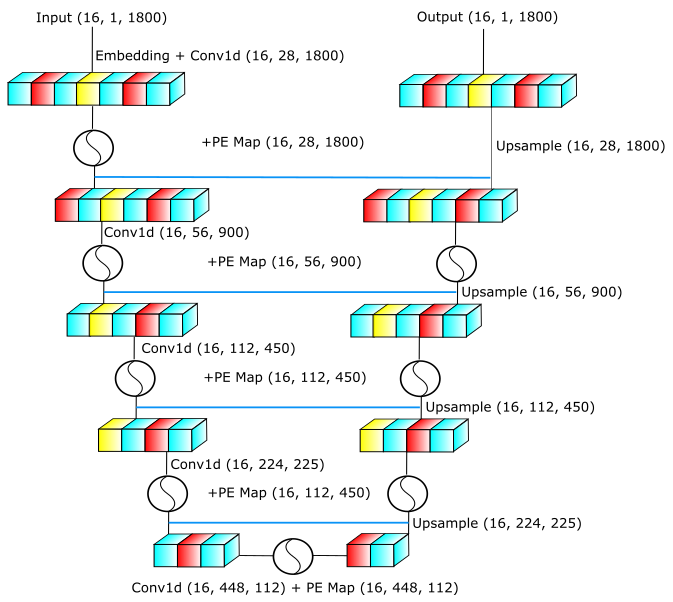
\includegraphics[width=0.7\linewidth]{ch6/figs/unet.png}
    \label{fig:cpunet}
    % \hspace{0.05\linewidth}
    \caption{Layer wise breakdown of the Positional U-Net. The blue lines represents the  skip connections between contracting and expanding paths of the U-Net. Positional encoding layers are also shown for all level. Credit: Aobo Li}
   \label{fig:network_schematic}
\end{figure}

%Unlike Reference~\cite{VAE}, we did not use  Kullback-Leibler Divergence to regulate the reparameterized random distribution.


\subsection{Positional U-Net}

We explored a U-Net~\cite{UNet}, a convolutional neural network initially developed for biomedical image segmentation, as the baseline model when designing the ATN. U-Net contains contracting (encoding) and expansive (decoding) channels. The contracting path contains $n$ convolutional layers to encode a waveform into a characteristic vector to capture contextual information and reduce the spatial resolution of the input. The expanding path contains $n$ upsample layers to decode the feature vector back to an output with the same length. The network structure also allows information to flow at different levels to the decoding part to provide maximum reconstruction efficiency. The U-Net structure is depicted in Figure ~\ref{fig:network_schematic}, where the tensor shape is also denoted at each stage. The Conv1d module in Figure~\ref{fig:network_schematic} is a series of layers whose breakdown is shown in Figure~\ref{ch6:fig:cov1d_break_down}. Within this module, the kernel size is an important hyperparameter to control the reception field of CNN layers, and padding is added to guarantee the same input and output shape. Max pooling is used in all Conv1d modules, but the first to increase the reception field. 

\begin{figure}[htb!]
    \centering
    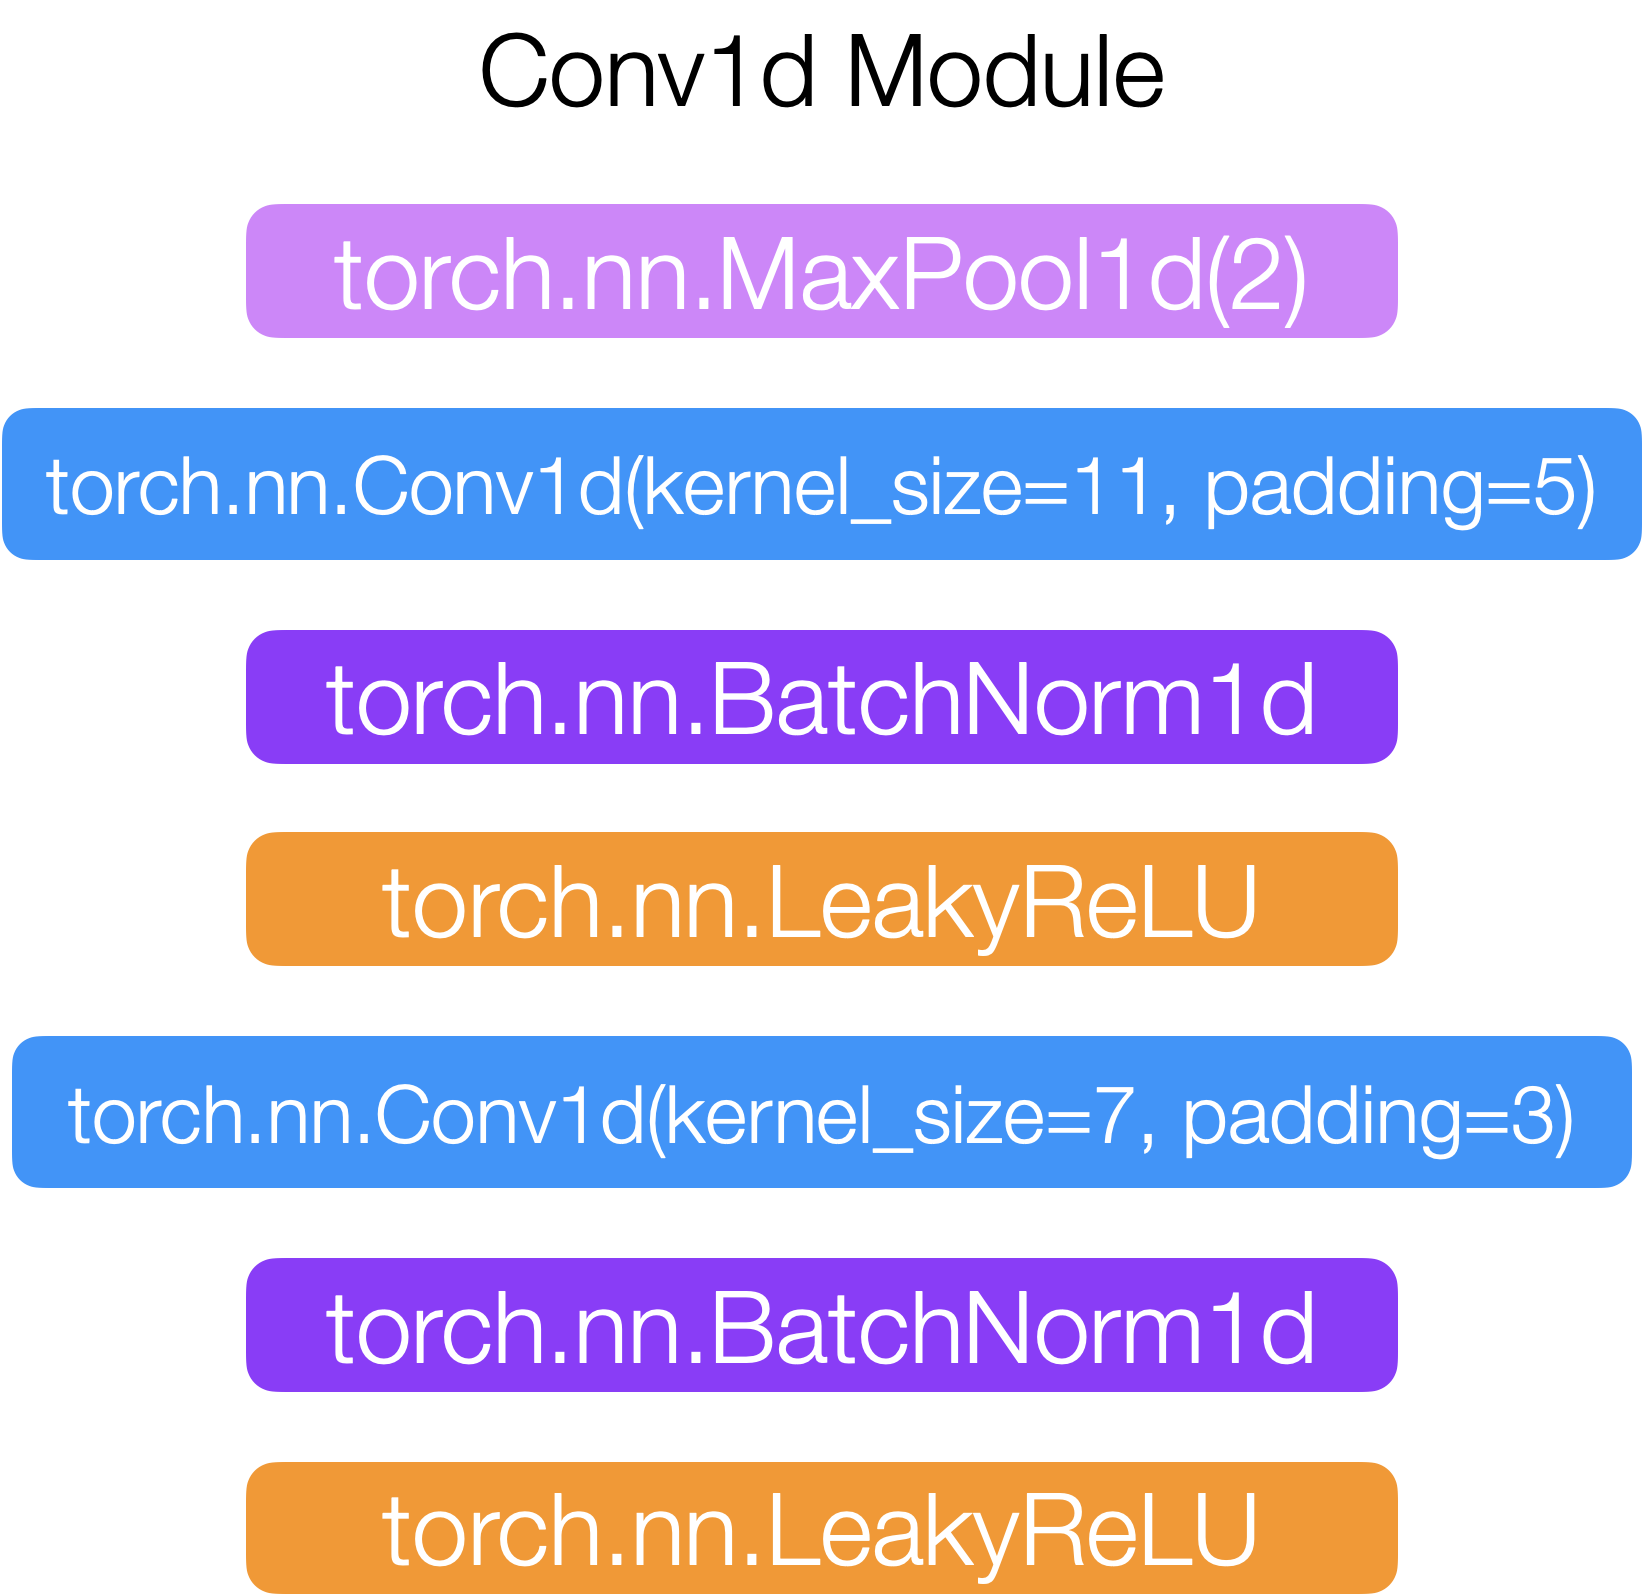
\includegraphics[width=0.3\linewidth,trim={0pc 0pc 0pc 0pc},clip]{ch6/figs/conv1d.png}
    \caption{Components of the Conv1d Module in the PU-Net from Figure~\ref{fig:network_schematic}.  Credit: Aobo Li}
    \label{ch6:fig:cov1d_break_down}
\end{figure}

During initial testing, it was observed that the traditional U-Net does not reproduce the tail of the waveform because of the lack of positional information in intermediate layer outputs. The Transformer model~\cite{Transformer} solves a similar problem by adding a positional encoding $\mathcal{M}_{\mathrm{position}}$ which contains sine and cosine functions with different frequencies to the output. The positional encoding in the Transformer model is given by:

\begin{equation}
PE_{(p, 2i)} = \sin\left(\frac{p}{10000^{\frac{2i}{d_{\text{ch}}}}}\right)
\label{eqn:positional_encoding_sin}
\end{equation}

\begin{equation}
PE_{(p, 2i+1)} = \cos\left(\frac{p}{10000^{\frac{2i}{d_{\text{ch}}}}}\right)
\label{eqn:positional_encoding_cos}
\end{equation}
where p is the position index of the token in the sequence, i is the dimension index and $d_{ch}$ is the dimension of input and output tensors. 10000 was the default value used in the transformer paper. We added the position encoding to the layers of U-Net to preserve the positional information at each stage. Since each U-Net layer outputs a tensor with a different shape, $\mathcal{M}_{\mathrm{position}}$ must be generated separately for each layer and added to the layer output, as shown in Figure~\ref{fig:network_schematic}.



Finally, we added a reparametrization trick to the bottom of PU-Net. The trick was developed in the Variational Autoencoder paper~\cite{VAE} to sample a random space while preserving the gradient flow. Reference~\cite{AAE} pointed out that this trick has the ability to increase the stochasticity of machine learning models. Based on our experiments, increased stochasticity helps the model learn the reconstruction features' distributions better. Together we call this model Positional U-Net~(PU-Net).

\subsection{RNN with Attention}~\label{subapp:RNN}
RNN is an ideal model for tasks involving time series data because the position is intrinsically enforced by RNN. \cite{Rumelhart1986} An RNN consists of recurrent neurons in which each neuron has an output and a hidden state, which is passed to the next-step neuron. Thus, the RNN remembers the previous time state and uses it for the current output; however, the RNN can suffer from the vanishing gradient problem, where the gradients used to update the network become very small and do not allow it to learn the long-range dependencies well across time steps. A Gated Recurrent Unit can help address this challenge by using "gates" that regulate the flow of information and gradients. ~\cite{GRU}. We developed a bidirectional RNN that adopts a Gated Recurrent Unit~\cite{GRU} as its internal structure.


\begin{figure}[htb!]
    \centering
    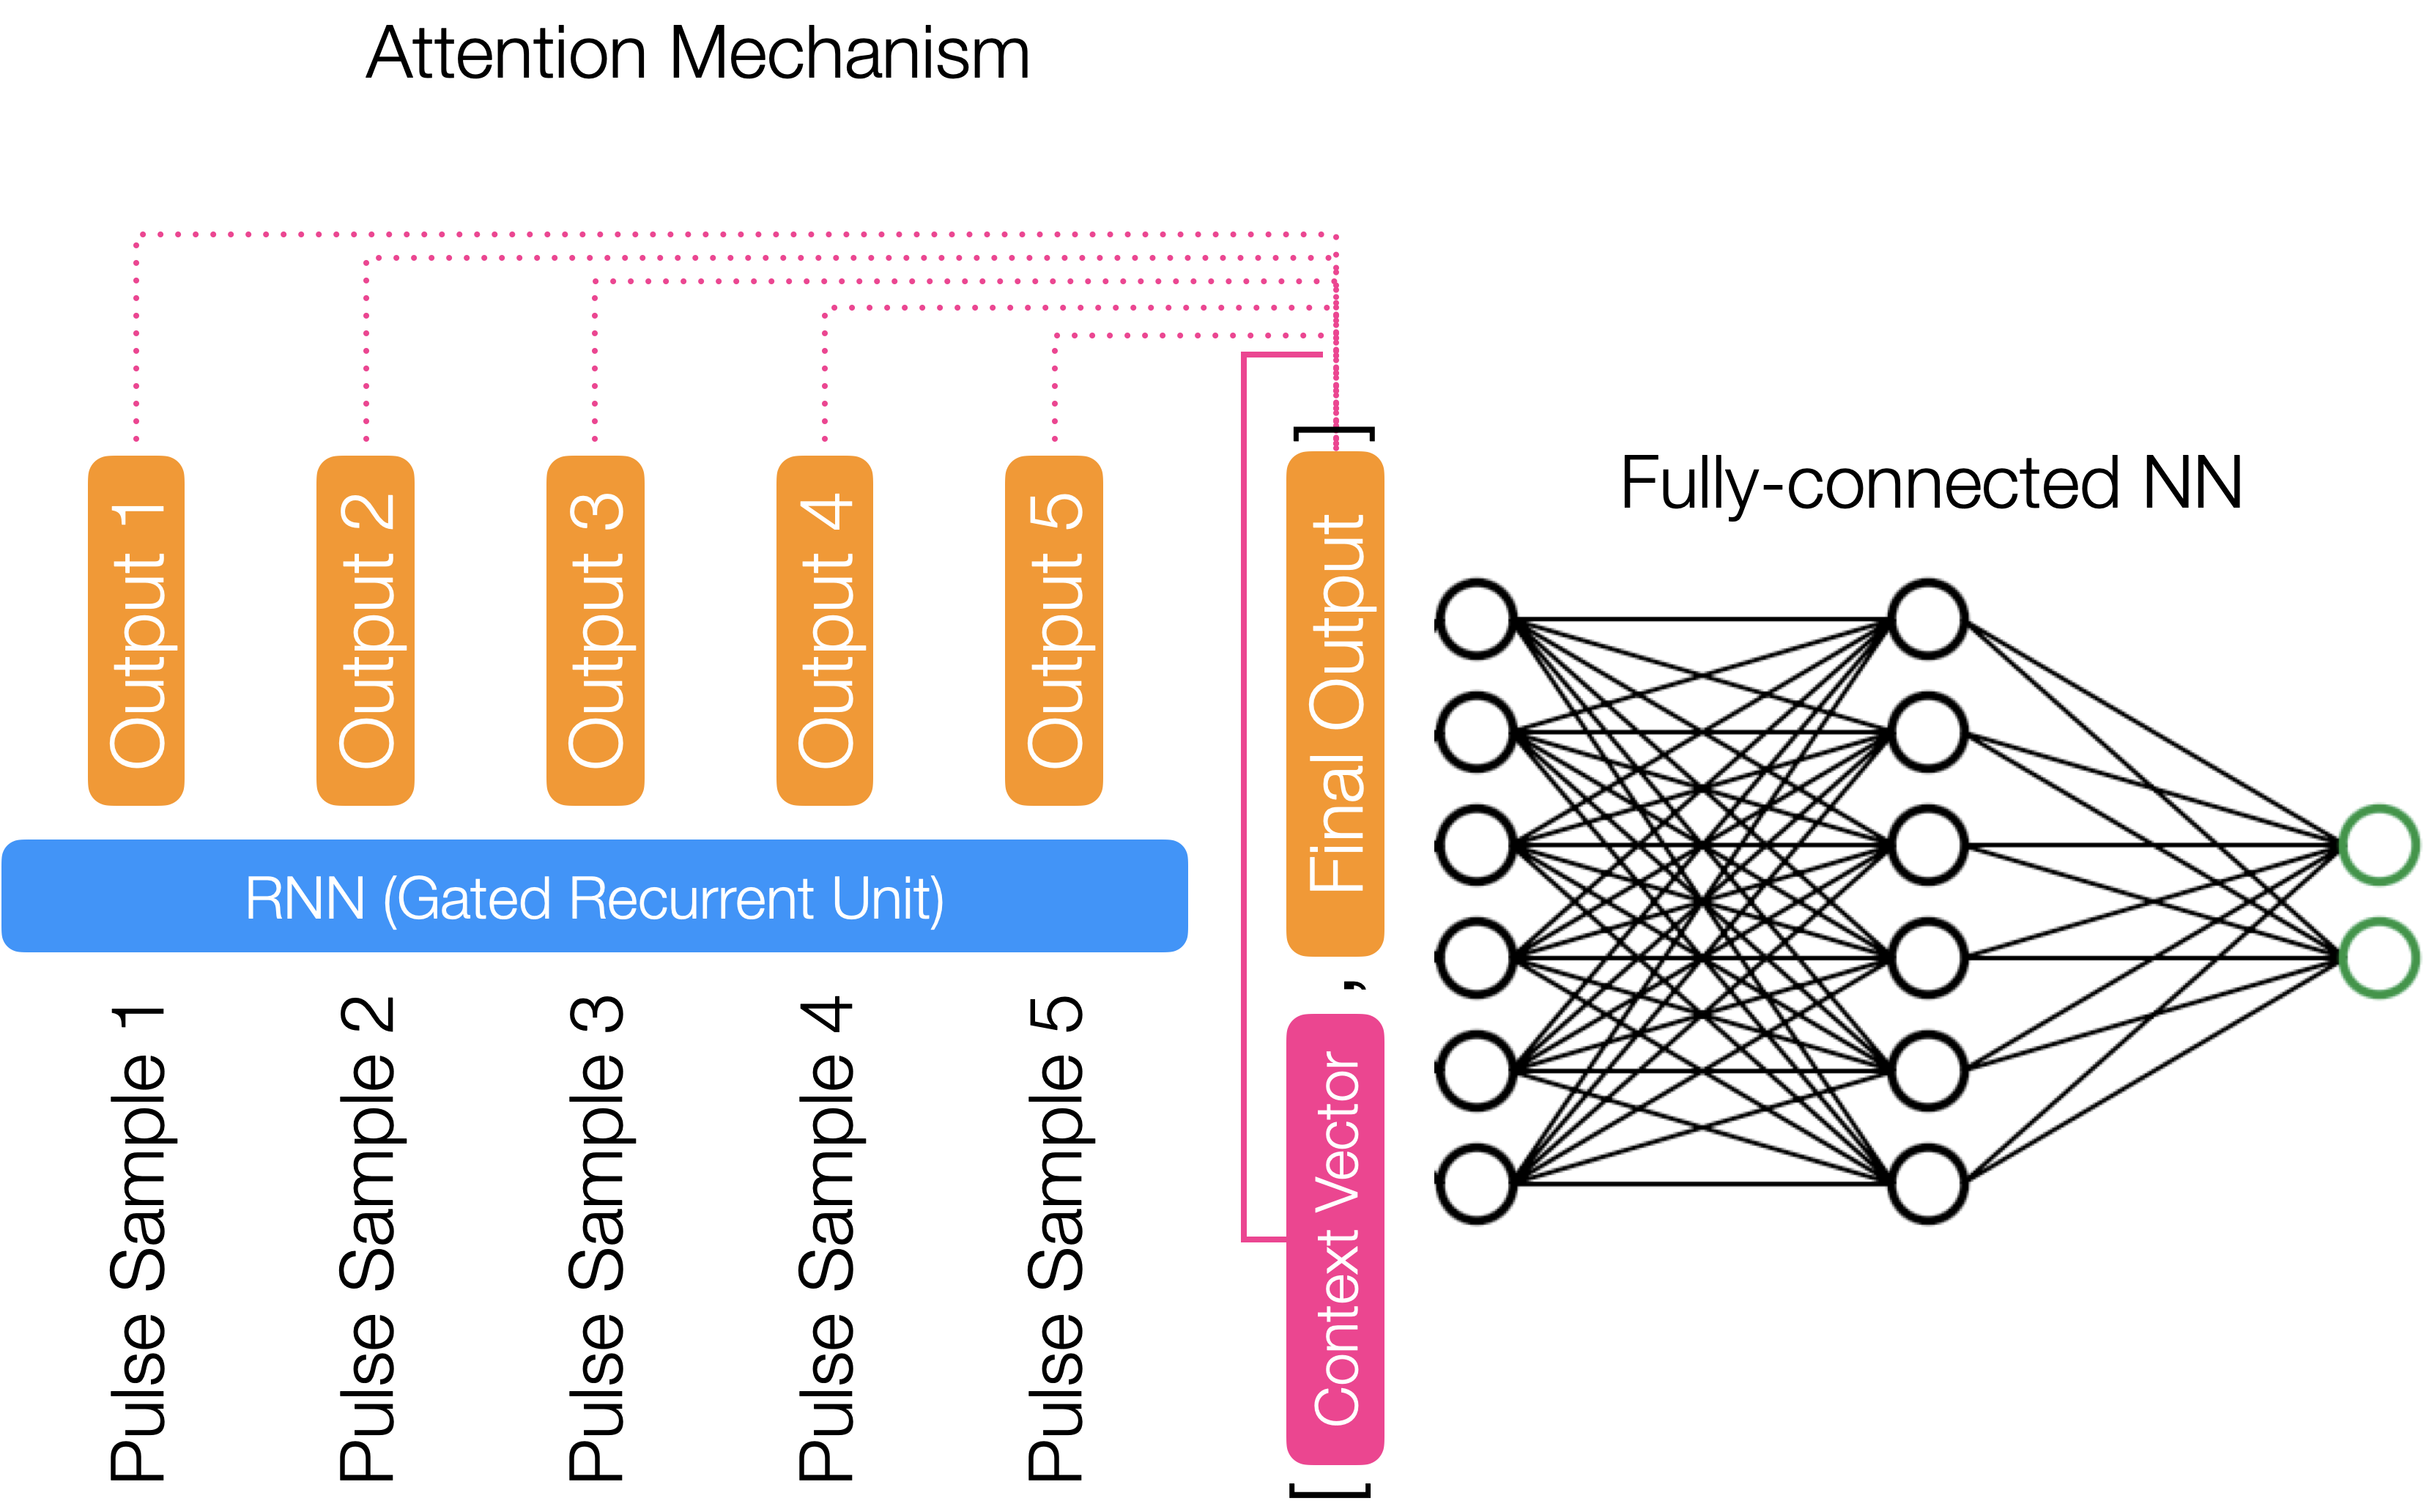
\includegraphics[width=0.7\linewidth,trim={0pc 0pc 0pc 0pc},clip]{ch6/figs/rnnAttention.png}
    \caption{The attention coupled RNN discriminator. Waveform are embedded into 128 dimension space and then passed to a GRU unit. The outputs of the GRU are used to calculate the attention score. The Final output along with the   The out Credit: Aobo Li}
    \label{ch6_fig_detail_network}
\end{figure}

The RNN model is shown in Figure\ref{ch6_fig_detail_network}. During training, the raw input waveforms are first embedded in the $m=128$ space. Embedding is done by initializing a lookup table that maps integer indices to dense vectors of fixed size. These vector representations are learned during training iterations to capture meaningful waveform features. We used an embedding trick that optimizes computation by directly retrieving the corresponding row from the embedding matrix instead of performing unnecessary matrix multiplications. 

The embedded waveform is fed into a GRU that processes them sequentially while maintaining hidden states to capture temporal dependencies. This yields a 64-dimensional output $\vec{I}(t)$ at each intermediate step $t$ as well as a final output $\vec{F}$. We then use an attention mechanism~\cite{attention} which can boost the performance of RNNs by allowing it to focus on different parts of the waveforms, such as the rising edge during different steps of the training. The attention mechanism contains an attention matrix A of dimension (64,64), which is used to calculate the attention score between $\vec{F}$ and each $\vec{I}(t)$. This calculates how much each time step contributes to the final output:
\begin{equation}
    s(t) = \mathrm{Softmax}[\vec{I}(t) A \vec{F}]
\end{equation}
A context vector is produced by summing $\vec{I}(t)$ with the weight $s(t)$ at each $t$. Finally, the context vector and the final output vector are concatenated and fed into a fully connected layer that produces a single-scalar output.

